\newgeometry{paper=a4paper, lmargin=0.1\paperwidth, rmargin=0.1\paperwidth, tmargin=1in, bmargin=1in}
\newpage
\begin{center}
    \thispagestyle{empty}

    \vspace*{4in}

    
    {\normalfont\sffamily\fontsize{36}\normalfont\itshape{Everything Science} \\ \vspace*{1cm}
     \normalfont\sffamily\fontsize{22}\normalfont\itshape{Grade 11 Physical Science}}
    \vspace*{1in} \\
    \LARGE Version 0.9 -- NCS \\

   {\vspace*{2in}
     by Siyavula and volunteers 
  

\vfill

    }
\end{center}






% Copyright notice
\newpage
\thispagestyle{empty}
\begin{center}
\normalfont\sffamily\fontsize{22}\normalfont\itshape Copyright notice\\

\vspace*{1in}

\textbf{Your freedom to legally copy this book}\\

\end{center}


{\LARGE
You are allowed and encouraged to freely copy this book. You can photocopy, print and distribute it as
often as you like. You can download it onto your mobile phone, iPad, PC or flash drive. You can burn it
to CD, e-mail it around or upload it to your website. \par

The only restriction is that you have to keep this book, its cover and short-codes unchanged.\par

For more information about the Creative Commons Attribution-NoDerivs 3.0 Unported (CC BY-ND
3.0) license see http://creativecommons.org/licenses/by-nd/3.0/}\\

\vspace*{4in}

\begin{center}
\begin{minipage}{0.6\textwidth}

\includegraphics[width=0.8\textwidth]{title_images/cc2.eps}
\end{minipage}
\begin{minipage}{0.3\textwidth}

\includegraphics[width=0.8\textwidth]{title_images/cc1.eps}
\end{minipage}
\end{center}







% Authors
\newpage
\thispagestyle{empty}


\begin{flushleft} \textbf{\huge Authors List} \end{flushleft}

{\LARGE This book is based upon the original Free High School Science Text which was entirely written by
volunteer academics, educators and industry professionals. Their vision was to see a curriculum aligned
set of mathematics and physical science textbooks which are freely available to anybody and exist
under an open copyright license.} \par

\textbf{\LARGE Siyavula core team} \\

Mark Horner; Heather Williams; René Toerien; Veena Maharaj; Marongwa Masemula; Elize Jones; Kevin Reddy; Marius Diergaard \par

\textbf{\LARGE Original Free High School Science Texts core team}\\

Mark Horner; Samuel Halliday; Sarah Blyth; Rory Adams; Spencer Wheaton \par 


\textbf{\LARGE Original Free High School Science Texts editors}\\

Jaynie Padayachee; Joanne Boulle; Diana Mulcahy; Annette Nell; René Toerien; Donovan Whitfield \par

\textbf{\LARGE Siyavula and Free High School Science Texts contributors}\\

    Sarah Abel;
Dr. Rory Adams;
    Andrea Africa;
    Matthew Amundsen;
    Ben Anhalt;
    Prashant Arora;
    Amos Baloyi;
    Bongani Baloyi;
    Raymond Barbour;
    Caro-Joy Barendse;
    Richard Baxter;
    Tara Beckerling;
Dr. Sarah Blyth;
    Sebastian Bodenstein;
    Martin Bongers;
    Gareth Boxall;
    Stephan Brandt;
    Hannes Breytenbach;
    Alex Briell;
    Wilbur Britz;
    Graeme Broster;
    Craig Brown;
    Richard Burge;
    Bianca Böhmer;
    George Calder-Potts;
    Eleanor Cameron;
    Richard Case;
    Sithembile Cele;
    Alice Chang;
    Richard Cheng;
    Fanny Cherblanc;
Dr. Christine Chung;
    Brett Cocks;
    Stefaan Conradie;
    Rocco Coppejans;
    Tim Craib;
    Andrew Craig;
    Tim Crombie;
    Dan Crytser;
Dr. Anne Dabrowski;
    Laura Daniels;
    Gareth Davies;
    Jennifer de Beyer;
    Jennifer de Beyer;
    Deanne de Bude;
    Mia de Vos;
    Sean Dobbs;
    Buhle Donga;
    William Donkin;
    Esmi Dreyer;
    Nicola du Toit;
    Matthew Duddy;
    Fernando Durrell;
Dr. Dan Dwyer;
    Alex Ellis;
    Tom Ellis;
    Andrew Fisher;
    Giovanni Franzoni;
    Nina Gitau Muchunu;
    Lindsay Glesener;
    Kevin Godby;
Dr. Vanessa Godfrey;
    Terence Goldberg;
Dr. Johan Gonzalez;
    Saaligha Gool;
    Hemant Gopal;
Dr. Stephanie Gould;
    Umeshree Govender;
    Heather Gray;
    Lynn Greeff;
    Carine Grobbelaar;
Dr. Tom Gutierrez;
    Brooke Haag;
    Kate Hadley;
    Alex Hall;
Dr. Sam Halliday;
    Asheena Hanuman;
Dr. Nicholas Harrison;
    Neil Hart;
    Nicholas Hatcher;
    Jason Hayden;
    Laura Hayward;
    Cho Hee Shrader;
Dr. Fritha Hennessy;
    Shaun Hewitson;
    Millie Hilgart;
    Grant Hillebrand;
    Nick Hobbs;
    Chris Holdsworth;
Dr. Benne Holwerda;
Dr. Mark Horner;
    Robert Hovden;
    Mfandaidza Hove;
    Jennifer Hsieh;
    Laura Huss;
Dr. Matina J. Rassias;
    Rowan Jelley;
    Grant Jelley;
    Clare Johnson;
    Luke Jordan;
    Tana Joseph;
Dr. Fabian Jutz;
    Brian Kamanzi;
Dr. Lutz Kampmann;
    Simon Katende;
    Natalia Kavalenia;
    Nothando Khumalo;
    Paul Kim;
Dr. Jennifer Klay;
    Lara Kruger;
    Sihle Kubheka;
    Andrew Kubik;
Dr. Jannie Leach;
    Nkoana Lebaka;
Dr. Tom Leinster;
    Henry Liu;
    Christopher Loetscher;
    Mike Loseby;
    Amandla Mabona;
    Malothe Mabutho;
    Stuart Macdonald;
Dr. Anton Machacek;
    Tshepo Madisha;
    Batsirai Magunje;
Dr. Komal Maheshwari;
    Michael Malahe;
    Masoabi Malunga;
    Masilo Mapaila;
    Bryony Martin;
    Nicole Masureik;
    John Mathew;
Dr. Will Matthews;
    Chiedza Matuso;
    JoEllen McBride;
    Dr Melanie Dymond Harper;
    Nikolai Meures;
    Riana Meyer;
    Filippo Miatto;
    Jenny Miller;
    Abdul Mirza;
    Mapholo Modise;
    Carla Moerdyk;
    Tshwarelo Mohlala;
    Relebohile Molaoa;
    Marasi Monyau;
    Asogan Moodaly;
    Jothi Moodley;
    Robert Moon;
    Calvin Moore;
    Bhavani Morarjee;
    Kholofelo Moyaba;
    Kate Murphy;
    Emmanuel Musonza;
    Tom Mutabazi;
    David Myburgh;
    Kamie Naidu;
    Nolene Naidu;
    Gokul Nair;
    Vafa Naraghi;
    Bridget Nash;
    Tyrone Negus;
    Huw Newton-Hill;
    Buntu Ngcebetsha;
Dr. Markus Oldenburg;
    Thomas O’Donnell;
Dr. William P. Heal;
Dr. Jaynie Padayachee;
    Poveshen Padayachee;
    Masimba Paradza;
    Dave Pawson;
    Justin Pead;
    Nicolette Pekeur;
    Sirika Pillay;
    Jacques Plaut;
    Barry Povey;
    Barry Povey;
    Andrea Prinsloo;
    Joseph Raimondo;
    Sanya Rajani;
    Alastair Ramlakan;
Dr. Jocelyn Read;
    Jonathan Reader;
    Jane Reddick;
Dr. Matthew Reece;
    Razvan Remsing;
    Laura Richter;
    Max Richter;
    Sean Riddle;
Dr. David Roberts;
    Christopher Roberts;
    Helen Robertson;
    Evan Robinson;
    Raoul Rontsch;
Dr. Andrew Rose;
    Katie Ross;
    Jeanne-Marié Roux;
    Mark Roux;
    Bianca Ruddy;
    Nitin Rughoonauth;
    Katie Russell;
    Steven Sam;
Dr. Carl Scheffler;
    Nathaniel Schwartz;
    Duncan Scott;
    Helen Seals;
    Relebohile Sefako;
    Prof. Sergey Rakityansky;
    Sandra Serumaga-Zake;
    Paul Shangase;
    Cameron Sharp;
    Ian Sherratt;
Dr. James Short;
    Roger Sieloff;
    Brandon Sim;
    Bonga Skozana;
    Clare Slotow;
    Bradley Smith;
    Greg Solomon;
    Nicholas Spaull;
Dr. Andrew Stacey;
Dr. Jim Stasheff;
    Mike Stay;
    Mike Stringer;
    Masixole Swartbooi;
    Tshenolo Tau;
    Tim Teatro;
    Ben Tho.epson;
    Shen Tian;
    Xolani Timbile;
    Robert Torregrosa;
    Jimmy Tseng;
    Tim van Beek;
    Neels van der Westhuizen;
    Frans van Eeden;
    Pierre van Heerden;
Dr. Marco van Leeuwen;
    Marina van Zyl;
    Pieter Vergeer;
    Rizmari Versfeld;
    Mfundo Vezi;
    Mpilonhle Vilakazi;
    Ingrid von Glehn;
    Tamara von Glehn;
    Kosma von Maltitz;
    Helen Waugh;
    Leandra Webb;
Dr. Dawn Webber;
    Michelle Wen;
Dr. Alexander Wetzler;
Dr. Spencer Wheaton;
    Vivian White;
Dr. Gerald Wigger;
    Harry Wiggins;
    Heather Williams;
    Wendy Williams;
    Julie Wilson;
    Timothy Wilson;
    Andrew Wood;
    Emma Wormauld;
Dr. Sahal Yacoob;
    Jean Youssef;
    Ewald Zietsman 




% Everything Maths page
\newpage
\thispagestyle{empty}

{\normalfont\sffamily\fontsize{22}\normalfont\itshape Everything Science} \par

{ \Large
When we look outside at everything in nature, look around us at everything manufactured or look up at everything in space we cannot but be struck by the incredible diversity and complexity of life; so many things, that look so different, operating in such unique ways. The physical universe really contains incredible complexity.\par

Yet, what is even more remarkable than this seeming complexity is the fact that things in the physical universe are knowable. We can investigate them, analyse them and understand them. It is this ability to understand the physical universe that allows us to transform elements and make technological progress possible.\par

If we look back at some of the things that developed over the last century – space travel, advances in medicine, wireless communication (from television to mobile phones) and materials a thousand times stronger than steel – we see they are not the consequence of magic or some inexplicable phenomena. They were all developed through the study and systematic application of the physical sciences. So as we look forward at the 21st century and some of the problems of poverty, disease and pollution that face us, it is partly to the physical sciences we need to turn. \par

For however great these challenges seem, we know that the physical universe is knowable and that the dedicated study thereof can lead to the most remarkable advances. There can hardly be a more exciting challenge than laying bare the seeming complexity of the physical universe and working with the incredible diversity therein to develop products and services that add real quality to people’s lives.\par

Physical sciences is far more wonderful, exciting and beautiful than magic! It is everywhere.

See introductory video by Dr. Mark Horner: \raisebox{-0.2em}{
\includegraphics[height=1em]{../../icons/video.ps}} VPsfk at www.everythingscience.co.za

}





% Webbook page

\newpage
\thispagestyle{empty}

{\normalfont\sffamily\fontsize{22}\normalfont\itshape More than a regular textbook} \par

\begin{center}
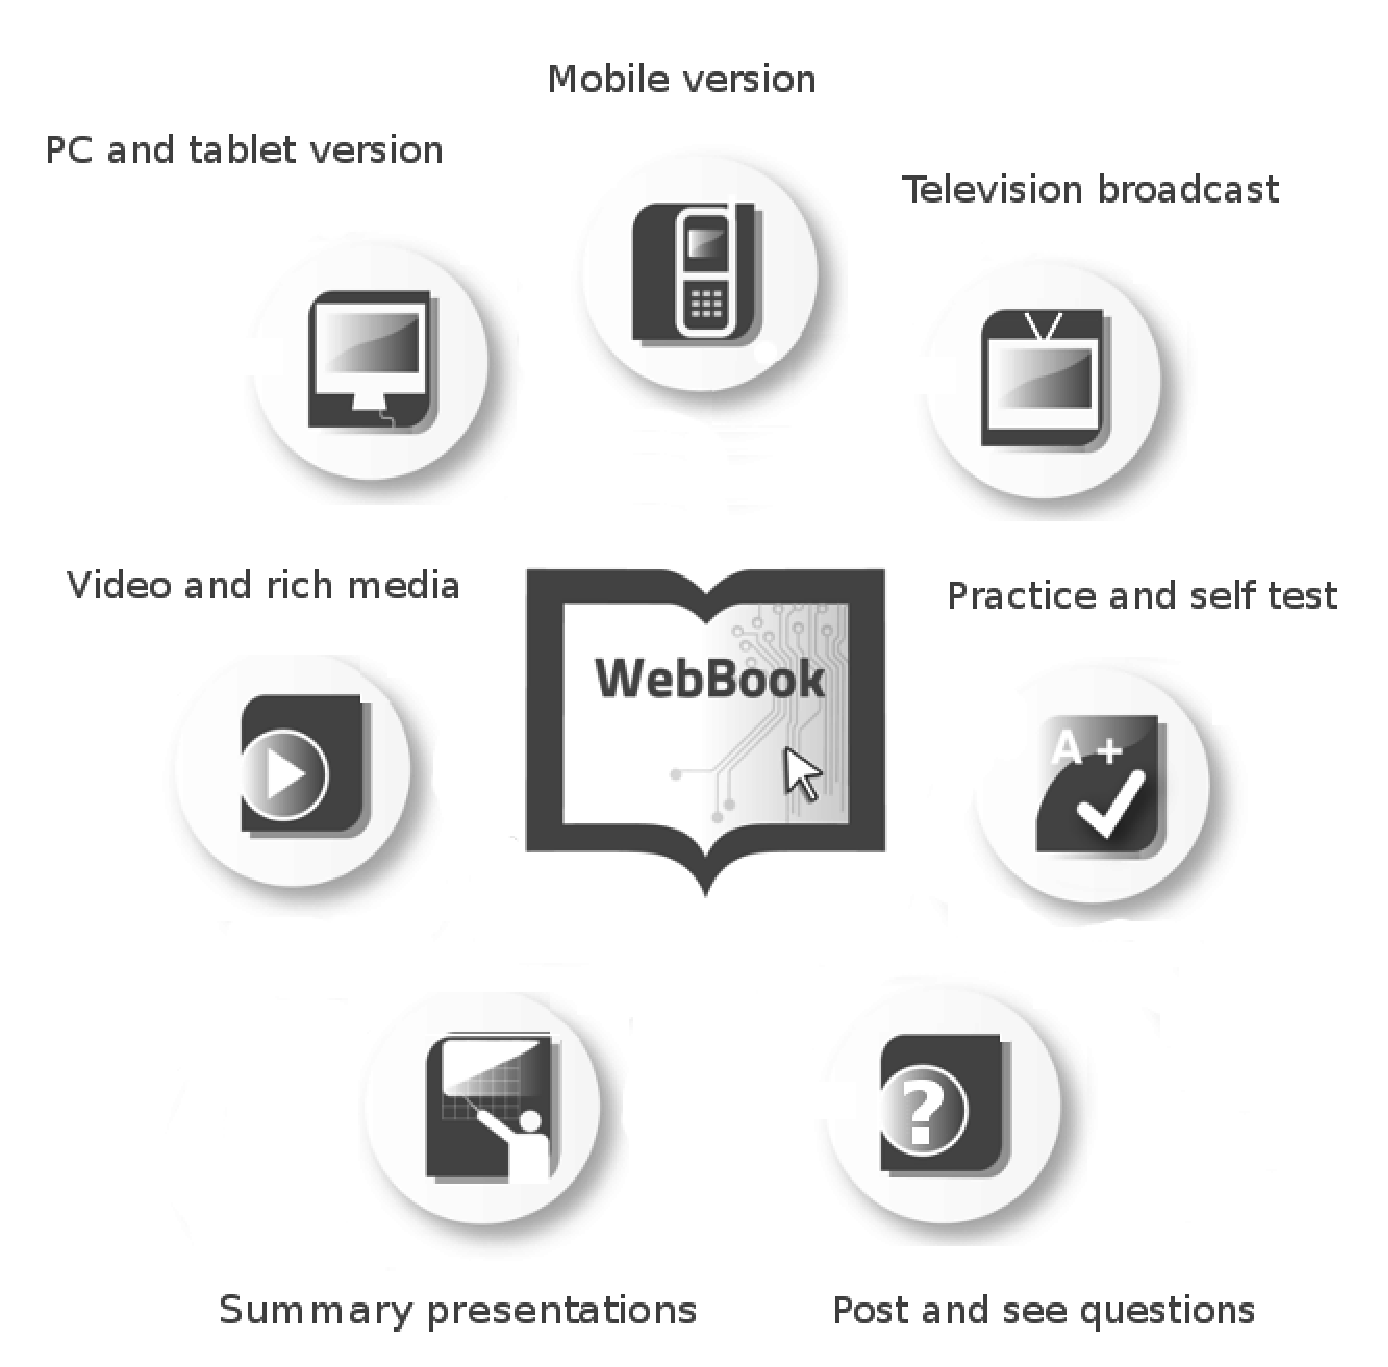
\includegraphics[width=0.70\textwidth]{title_images/morethantextbook.eps}
\end{center}

\par
{\Large
\textbf{\textit{Everything Science}} is not just a Science textbook. It has everything you expect from
your regular printed school textbook, but comes with a whole lot more. For a start, you can download or read it
on-line on your mobile phone, computer or iPad, which means you have the convenience of accessing
it wherever you are.\par


We know that some things are hard to explain in words. That is why every chapter comes with video
lessons and explanations which help bring the ideas and concepts to life. Summary presentations at
the end of every chapter offer an overview of the content covered, with key points highlighted for easy
revision.\par


All the exercises inside the book link to a service where you can get more practice, see the full solution
or test your skills level on mobile and PC.\par


We are interested in what you think, wonder about or struggle with as you read through the book and
attempt the exercises. That is why we made it possible for you to use your mobile phone or computer to
digitally pin your question to a page and see what questions and answers other readers pinned up.\par


This book is the same one used by Mindset Learn in their new television broadcast, where experienced educators work through it, explain the concepts and work out exercises from the book.
}




% mobile or PC
\newpage
\thispagestyle{empty}

{\normalfont\sffamily\fontsize{22}\normalfont\itshape Everything Science on your mobile or PC} \par

{\Large
You can have this textbook at hand wherever you are – whether at home, on the the train or at school.
Just browse to the on-line version of Everything Science on your mobile phone, tablet or computer. To
read it off-line you can download a PDF or e-book version.\par


To read or download it, go to \textbf{www.everythingscience.co.za} on your phone or computer.} \vspace*{2cm}


\begin{center}
\begin{minipage}{0.4\textwidth}
\centering
\includegraphics[width=0.8\textwidth]{title_images/ipad.eps}
\end{minipage}
\begin{minipage}{0.4\textwidth}
\centering
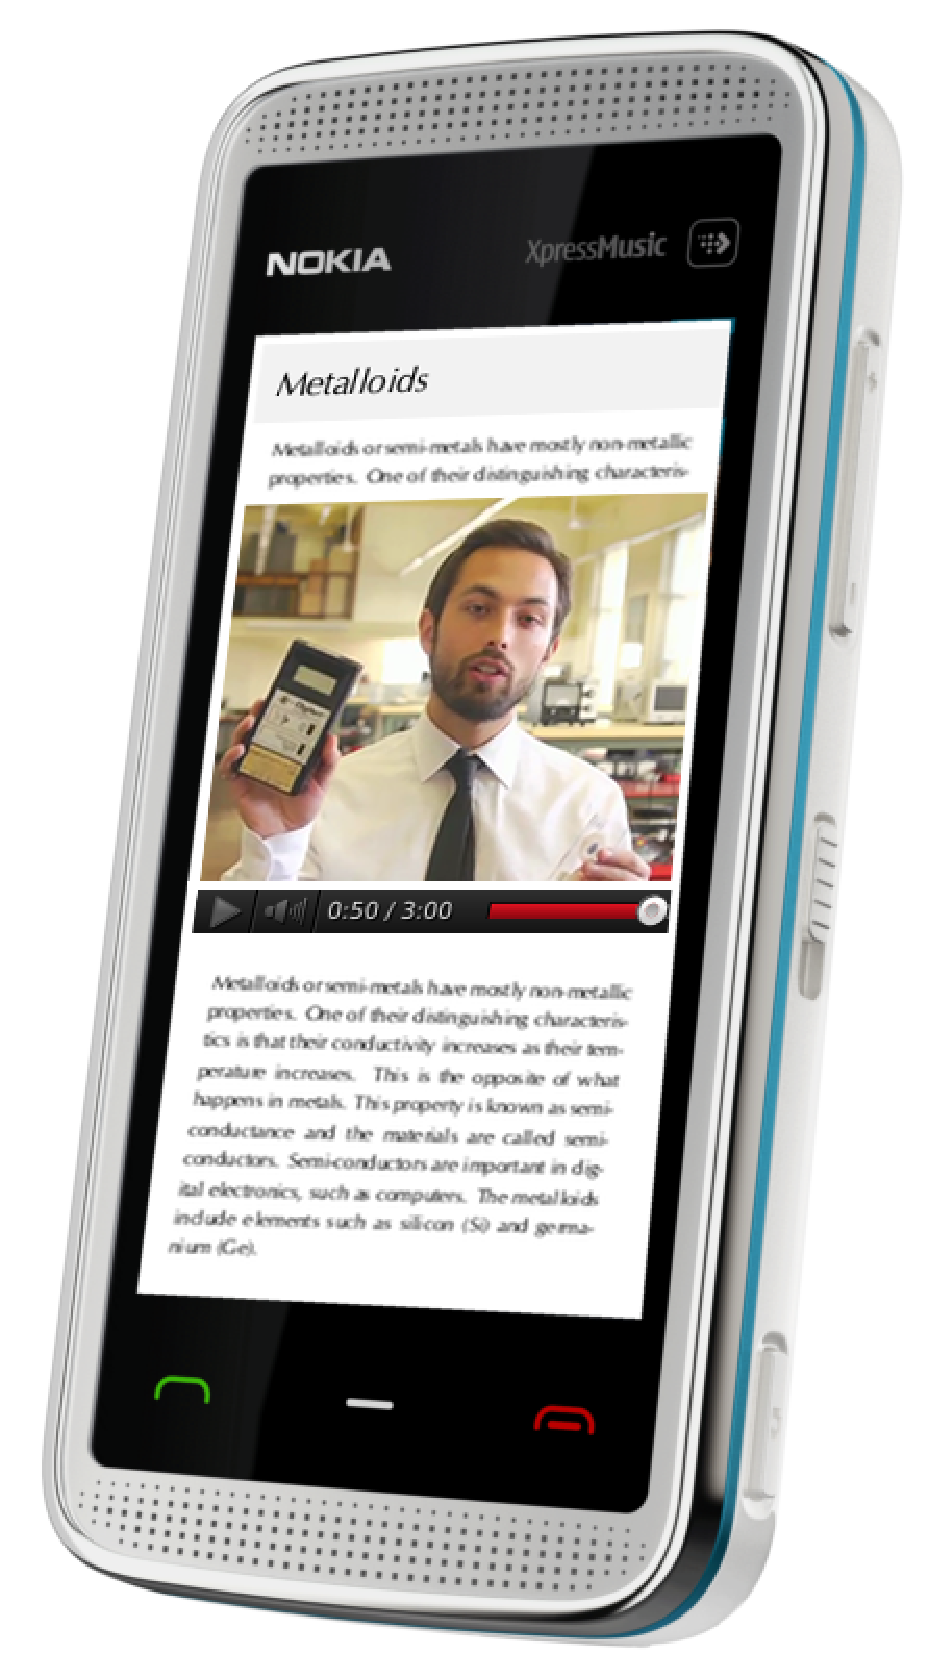
\includegraphics[width=0.4\textwidth]{title_images/phone.eps}
\end{minipage}
\end{center}

\vspace*{2cm}


{\normalfont\sffamily\fontsize{22}\normalfont\itshape Using the icons and short-codes} \par

{\Large
Inside the book you will find these icons to help you spot where videos, presentations, practice tools
and more help exist. The short-codes next to the icons allow you to navigate directly to the resources
on-line without having to search for them.\par


\begin{tabular}{lcl}
\raisebox{-0.8em}{
\includegraphics[width=0.8cm]{../../icons/www.ps}} & (A123) & Go directly to a section \\
\raisebox{-0.8em}{
\includegraphics[width=0.8cm]{../../icons/video.ps}} & (V123) & Video, simulation or presentation \\
\raisebox{-0.8em}{
\includegraphics[width=0.8cm]{../../icons/aplus.ps}} & (P123) & Practice and test your skills \\
\raisebox{-0.8em}{
\includegraphics[width=0.8cm]{../../icons/help.ps}} & (Q123) & Ask for help or find an answer \\
\end{tabular}
\par
\vspace*{1cm}

To watch the videos on-line, practise your skills or post a question, go to the \textit{Everything Science} website at \textbf{www.everythingscience.co.za} on your mobile or PC and enter the short-code in the navigation box.
}




% video lessons
\newpage
\thispagestyle{empty}

{\normalfont\sffamily\fontsize{22}\normalfont\itshape Video lessons} \par

{\Large

Look out for the video icons inside the book. These will take you to video lessons created by \textit{Mindset
Learn} that help bring the ideas and concepts on the page to life. Get extra insight, detailed
explanations and worked examples. See the concepts in action and hear real people talk about how they
use maths and science in their work. \par

\begin{center}
See video explanation \raisebox{-0.6em}{
\includegraphics[width=0.7cm]{../../icons/video.ps}} (Video: V123)\\
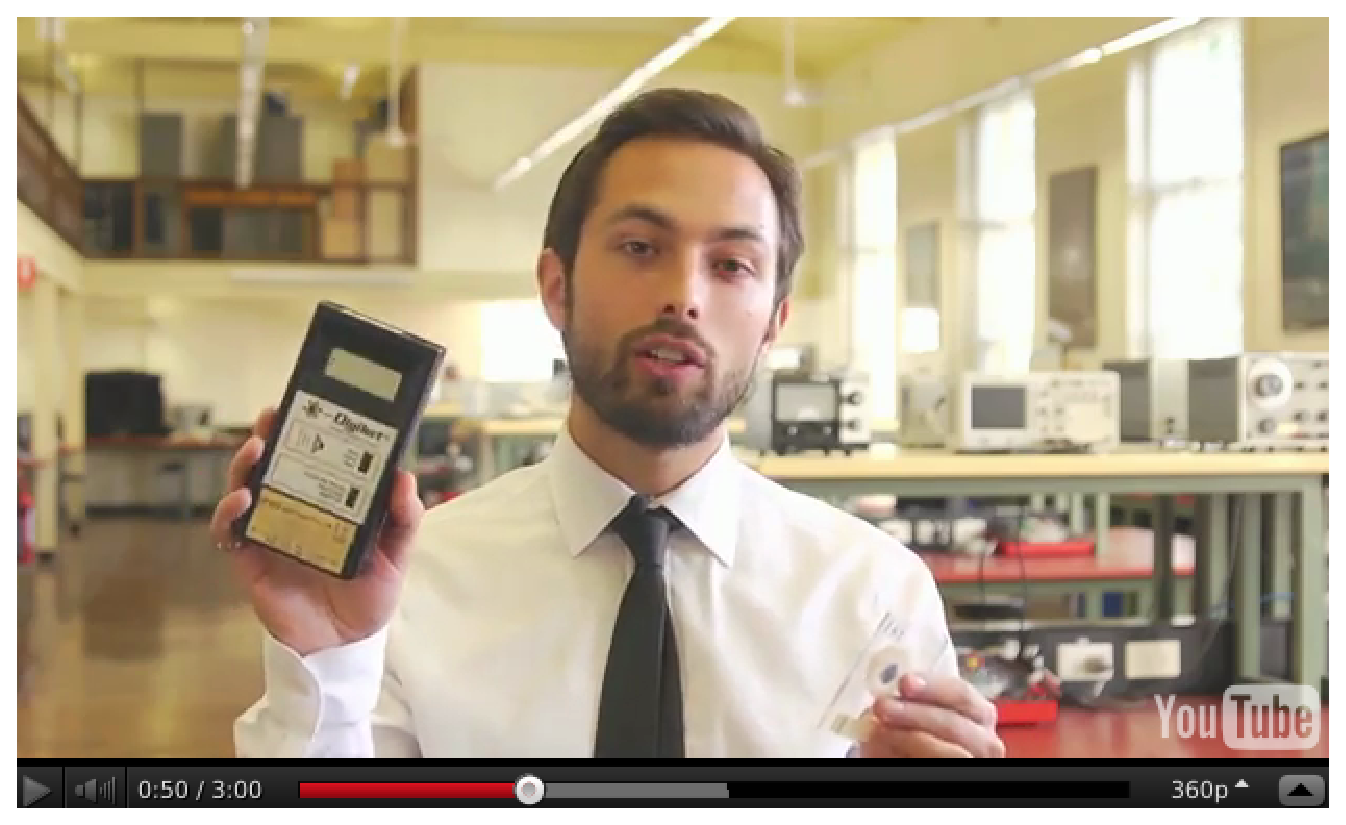
\includegraphics[width=0.5\textwidth]{title_images/veritasiumvideo.eps}
\end{center}\par

}
\vspace{0.5cm}
{\normalfont\sffamily\fontsize{22}\normalfont\itshape Video exercises} \par

{\Large

Wherever there are exercises in the book you will see icons and short-codes for video solutions,
practice and help. These short-codes will take you to video solutions of select exercises to show you
step-by-step how to solve such problems. \par

\begin{center}
See video exercise \raisebox{-0.6em}{
\includegraphics[width=0.7cm]{../../icons/video.ps}} (Video: V123) \\
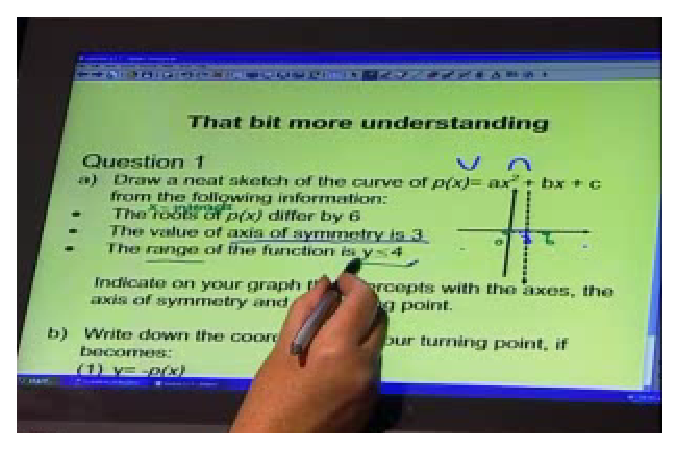
\includegraphics[width=0.5\textwidth]{title_images/mindsetexercise.eps}
\end{center}
\par
You can get these videos by:
\begin{itemize}
    \item viewing them on-line on your mobile or computer
    \item downloading the videos for off-line viewing on your phone or computer
    \item ordering a DVD to play on your TV or computer
    \item downloading them off-line over Bluetooth or Wi-Fi from select outlets
\end{itemize}
}


% practise and test your skills
\newpage
\thispagestyle{empty}
{\Large

To view, download, or for more information, visit the Everything Science website on your phone or
computer at \underline{www.everythingscience.co.za}  \par
\vspace*{1cm}
{\normalfont\sffamily\fontsize{22}\normalfont\itshape Practice and test your skills} \par


One of the best ways to prepare for your tests and exams is to practice answering the same kind of
questions you will be tested on. At every set of exercises you will see a practice icon and short-code.
This on-line practice for \textbf{mobile} and \textbf{PC} will keep track of your performance and progress, give you
feedback on areas which require more attention and suggest which sections or videos to look at.

\begin{center}
See more practice \raisebox{-0.6em}{
\includegraphics[width=0.7cm]{../../icons/aplus.ps}} (QM123) \\
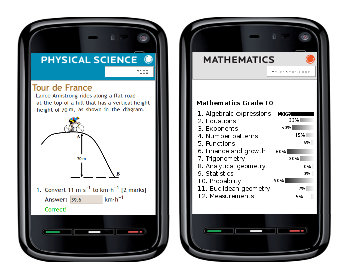
\includegraphics[width=0.65\textwidth]{title_images/practicephones.eps}
\end{center}
\par



To practice and test your skills:\par

Go to \underline{www.everythingscience.co.za} on your mobile phone or PC and enter the short-code.\par

\vspace*{1cm}


%{\normalfont\sffamily\fontsize{22}\normalfont\itshape Television broadcasts} \par
%This book is the same one used by \textbf{Mindset Learn} in their television broadcast where experienced
%educators explain the key concepts, perform live experiments and work out exercises from the book.
%\textbf{Mindset Learn} broadcasts a full 28 hours of curriculum support each week of term. \par
%
%
%Maths can be seen on Mondays and Science on Tuesdays. There is also Life Sciences on Wednesdays
%and Maths Literacy on Thursdays. Revision of the week's work is done on Saturdays for Grade 12 and on
%Sundays for Grades 10 and 11.
%

}

\newpage
\thispagestyle{empty}

{\normalfont\sffamily\fontsize{22}\normalfont\itshape Ask questions and find answers} \par

{\Large

Have you ever had a question about a specific fact, formula or exercise in your textbook and wished you could just ask someone? Surely someone else in the country must have had the same question at the same place in the textbook.\par 

We invite you to open the textbook on your mobile phone or computer and pin your question at that  exact spot in the textbook using the shortcode. You will be able to see whether it has been asked before and what the given answer to that question is. \par

The short codes at section headings helps you navigate to sections in the book to ask and view questions for that section. The short codes for the exercises lets you look at questions and answers relating to those specific exercises.\par

\begin{tabular}{lcl}
\raisebox{-0.8em}{
\includegraphics[width=0.8cm]{../../icons/www.ps}} & (A123) & Visit this section to post or view questions\\
\raisebox{-0.8em}{
\includegraphics[width=0.8cm]{../../icons/help.ps}} & (Q123) & Questions or help with a specific question  \\
\end{tabular}



\begin{figure}[h]
\centering
\includegraphics[width=\textwidth]{title_images/questions.eps}
\end{figure}


}
%

%
%% practise and test your skills
%\newpage
%\thispagestyle{empty}
%{\Large
%
%\begin{table*}[h]
%\large
%\begin{tabular}{lll}
%\textbf{Maths and Science Broadcasts}&&\\
%Grade 10  Maths & Mondays at 4pm & Every second Sunday at 1pm\\
%Grade 11  Maths & Mondays at 5pm & Every second Sunday at 9am\\
%Grade 12  Maths & Mondays at 6pm & Every Saturday at 9am\\
%Grade 10  Science & Tuesdays at 4pm & Every second Sunday at 1pm\\
%Grade 11  Science & Tuesdays at 5pm & Every second Sunday at 9am\\
%Grade 12  Science & Tuesdays at 6pm & Every Saturday at 11am\\
%\textbf{Other broadcasts} & & \\
%Grade 10  Life Science & Wednesdays at 4pm & Every second Sunday at 3pm\\
%Grade 11  Life Science & Wednesdays at 5pm & Every second Sunday at 9am\\
%Grade 12  Life Science & Wednesdays at 6pm & Every Saturday at 1pm\\
%Grade 10  Maths Literacy & Thursdays at 4pm & Every second Sunday at 3pm\\
%Grade 11  Maths Literacy & Thursdays at 5pm & Every second Sunday at 9am\\
%Grade 12  Maths Literacy & Thursdays at 6pm & Every Saturday at 3pm\\
%\end{tabular}
%\end{table*}
%
%
%\textbf{You can watch these live sessions on:}
%\begin{itemize}
%    \item Mindset free-to-air for schools (ask your school)
%    \item Channels 319 on DStv
%    \item Toptv on 319 on TopTV
%\end{itemize}


%}

% Put the margins back for the rest of the book

\newgeometry{lmargin=0.1\paperwidth, rmargin=0.25\paperwidth, tmargin=1in, bmargin=1in, twoside, centering, includehead,  marginparwidth=0.225\paperwidth}

\normalfont
